
%% Gravity Questions used on the
%% NYSED Physics Regents Examination
%%--------------------------------------------------

%% this section contains 72 problems


%% Section June2015
%%--------------------
\element{nysed}{
\begin{question}{June2015-Q11}
    The Hubble telescope's orbit is \SI{5.6e5}{\meter} above Earth's surface. 
    The telescope has a mass of \SI{1.1e4}{\kilo\gram}.
    Earth exerts a gravitational force of \SI{9.1e4}{\newton} on the telescope. 
    The magnitude of Earth's gravitational field strength at this location is:
    \begin{multicols}{2}
    \begin{choices}
        \wrongchoice{\SI{1.5e-20}{\newton\per\kilo\gram}}
        \wrongchoice{\SI{0.12}{\newton\per\kilo\gram}}
      \correctchoice{\SI{8.3}{\newton\per\kilo\gram}}
        \wrongchoice{\SI{9.8}{\newton\per\kilo\gram}}
    \end{choices}
    \end{multicols}
\end{question}
}


%% Section June2014
%%--------------------
\element{nysed}{
\begin{question}{June2014-Q06}
    A \SI{2.0}{\kilo\gram} mass is located \SI{3.0}{\meter} above the surface of Earth.
    What is the magnitude of Earth's gravitational field strength at this location?
    \begin{multicols}{2}
    \begin{choices}
      \correctchoice{\SI{9.8}{\newton\per\kilo\gram}}
        \wrongchoice{\SI{4.9}{\newton\per\kilo\gram}}
        \wrongchoice{\SI{2.0}{\newton\per\kilo\gram}}
        \wrongchoice{\SI{20.}{\newton\per\kilo\gram}}
    \end{choices}
    \end{multicols}
\end{question}
}


%% Section June2013
%%--------------------
\element{nysed}{
\begin{question}{June2013-Q13}
    At a certain location, a gravitational force with a magnitude of \SI{350}{\newton} acts on a \SI{70}{\kilo\gram} astronaut.
    What is the magnitude of the gravitational field strength at this location?
    \begin{multicols}{2}
    \begin{choices}
        \wrongchoice{\SI{0.20}{\kilo\gram\per\newton}}
      \correctchoice{\SI{5.0}{\newton\per\kilo\gram}}
        \wrongchoice{\SI{9.8}{\meter\per\second\squared}}
        \wrongchoice{\SI{25 000}{\newton\kilo\gram}}
    \end{choices}
    \end{multicols}
\end{question}
}

\element{nysed}{
\begin{question}{June2013-Q47}
    Which graph represents the relationship between the magnitude of the gravitational force between two masses and the distance between the centers of the masses?
    \begin{multicols}{2}
    \begin{choices}
        \AMCboxDimensions{down=-2.5em}
        \correctchoice{
            \begin{tikzpicture}
                \begin{axis}[
                    axis y line=left,
                    axis x line=bottom,
                    axis line style={->},
                    xlabel={distance},
                    xtick=\empty,
                    ylabel={force},
                    ytick=\empty,
                    xmin=0,xmax=11,
                    ymin=0,ymax=11,
                    width=\columnwidth,
                    very thin,
                ]
                \addplot[line width=1pt,domain=0:10]{10/x};
                \end{axis}
            \end{tikzpicture}
        }
        \wrongchoice{
            \begin{tikzpicture}
                \begin{axis}[
                    axis y line=left,
                    axis x line=bottom,
                    axis line style={->},
                    xlabel={distance},
                    xtick=\empty,
                    ylabel={force},
                    ytick=\empty,
                    xmin=0,xmax=11,
                    ymin=0,ymax=11,
                    width=\columnwidth,
                    very thin,
                ]
                \addplot[line width=1pt,domain=0:10]{x};
                \end{axis}
            \end{tikzpicture}
        }
        \wrongchoice{
            \begin{tikzpicture}
                \begin{axis}[
                    axis y line=left,
                    axis x line=bottom,
                    axis line style={->},
                    xlabel={distance},
                    xtick=\empty,
                    ylabel={force},
                    ytick=\empty,
                    xmin=0,xmax=11,
                    ymin=0,ymax=11,
                    width=\columnwidth,
                    very thin,
                ]
                \addplot[line width=1pt,domain=0:10]{10-x};
                \end{axis}
            \end{tikzpicture}
        }
        \wrongchoice{
            \begin{tikzpicture}
                \begin{axis}[
                    axis y line=left,
                    axis x line=bottom,
                    axis line style={->},
                    xlabel={distance},
                    xtick=\empty,
                    ylabel={force},
                    ytick=\empty,
                    xmin=0,xmax=11,
                    ymin=0,ymax=11,
                    width=\columnwidth,
                    very thin,
                ]
                \addplot[line width=1pt,domain=0:10]{0.1*x*x};
                \end{axis}
            \end{tikzpicture}
        }
    \end{choices}
    \end{multicols}
\end{question}
}


%% Section June2012
%%--------------------
\element{nysed}{
\begin{question}{June2012-Q42}
    Which graph represents the relationship between the magnitude of the gravitational force exerted by Earth on a spacecraft and the distance between the center of the spacecraft and center of Earth?
    Assume constant mass for the spacecraft.
    \begin{multicols}{2}
    \begin{choices}
        %% NOTE: Same as June2013-Q47
        \AMCboxDimensions{down=-2.5em}
        \correctchoice{
            \begin{tikzpicture}
                \begin{axis}[
                    axis y line=left,
                    axis x line=bottom,
                    axis line style={->},
                    xlabel={distance},
                    xtick=\empty,
                    ylabel={force},
                    ytick=\empty,
                    xmin=0,xmax=11,
                    ymin=0,ymax=11,
                    width=\columnwidth,
                    very thin,
                ]
                \addplot[line width=1pt,domain=0:10]{10/x};
                \end{axis}
            \end{tikzpicture}
        }
        \wrongchoice{
            \begin{tikzpicture}
                \begin{axis}[
                    axis y line=left,
                    axis x line=bottom,
                    axis line style={->},
                    xlabel={distance},
                    xtick=\empty,
                    ylabel={force},
                    ytick=\empty,
                    xmin=0,xmax=11,
                    ymin=0,ymax=11,
                    width=\columnwidth,
                    very thin,
                ]
                \addplot[line width=1pt,domain=0:10]{x};
                \end{axis}
            \end{tikzpicture}
        }
        \wrongchoice{
            \begin{tikzpicture}
                \begin{axis}[
                    axis y line=left,
                    axis x line=bottom,
                    axis line style={->},
                    xlabel={distance},
                    xtick=\empty,
                    ylabel={force},
                    ytick=\empty,
                    xmin=0,xmax=11,
                    ymin=0,ymax=11,
                    width=\columnwidth,
                    very thin,
                ]
                \addplot[line width=1pt,domain=0:10]{10-x};
                \end{axis}
            \end{tikzpicture}
        }
        \wrongchoice{
            \begin{tikzpicture}
                \begin{axis}[
                    axis y line=left,
                    axis x line=bottom,
                    axis line style={->},
                    xlabel={distance},
                    xtick=\empty,
                    ylabel={force},
                    ytick=\empty,
                    xmin=0,xmax=11,
                    ymin=0,ymax=11,
                    width=\columnwidth,
                    very thin,
                ]
                \addplot[line width=1pt,domain=0:10]{0.1*x*x};
                \end{axis}
            \end{tikzpicture}
        }
    \end{choices}
    \end{multicols}
\end{question}
}

\element{nysed}{
\begin{question}{June2012-Q48}
    In which diagram do the field lines best represent the gravitational field around the Earth?
    \begin{multicols}{2}
    \begin{choices}
        \AMCboxDimensions{down=-1.0cm}
        \correctchoice{
            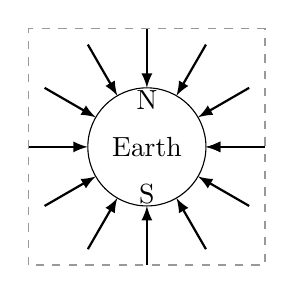
\begin{tikzpicture}
                \draw[dashed,white!60!black] (-1.5,-1.5) rectangle (1.5,1.5);
                \def\r{0.75}
                %% Earth
                \node[anchor=center] at (0,0) {Earth};
                \draw (0,0) circle (\r);
                %% labels
                \foreach \x/\y in {90/N,270/S} \node[anchor=center,shift={(\x:-1ex)}] at (\x:\r) {\y};
                %% field lines
                \foreach \x in {0,30,...,360} \draw[thick,latex-] (\x:\r) -- (\x:1.5);
            \end{tikzpicture}
        }
        \wrongchoice{
            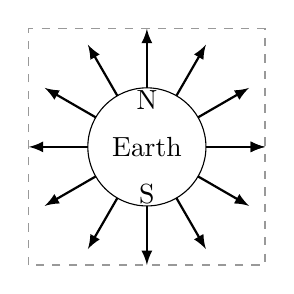
\begin{tikzpicture}
                \draw[dashed,white!60!black] (-1.5,-1.5) rectangle (1.5,1.5);
                \def\r{0.75}
                %% Earth
                \node[anchor=center] at (0,0) {Earth};
                \draw (0,0) circle (\r);
                %% labels
                \foreach \x/\y in {90/N,270/S} \node[anchor=center,shift={(\x:-1ex)}] at (\x:\r) {\y};
                %% field lines
                \foreach \x in {0,30,...,360} \draw[thick,-latex] (\x:\r) -- (\x:1.5);
            \end{tikzpicture}
        }
        \wrongchoice{
            \begin{tikzpicture}
                \draw[dashed,white!60!black] (-1.5,-1.5) rectangle (1.5,1.5);
                \def\r{0.75}
                %% Earth
                \node[anchor=center] at (0,0) {Earth};
                \draw (0,0) circle (\r);
                %% labels
                \foreach \x/\y in {90/N,270/S} \node[anchor=center,shift={(\x:-1ex)}] at (\x:\r) {\y};
                %% field lines
                \begin{scope}[decoration={markings,mark=at position 0.33 with {\arrow{latex}}}]
                    \clip (-1.5,-1.5) rectangle (1.5,1.5);
                    \foreach \x/\y in {20/2,40/1} {
                        \draw[thick,-latex,postaction={decorate}] ({270-\x}:0.75) .. controls ++(240:\y) and ++(130:\y) .. ({90+\x}:0.75);
                        \draw[thick,-latex,postaction={decorate}] ({270+\x}:0.75) .. controls ++(300:\y) and ++(60:\y) .. ({90-\x}:0.75);
                    }
                \end{scope}
            \end{tikzpicture}
        }
        \wrongchoice{
            \begin{tikzpicture}
                \draw[dashed,white!60!black] (-1.5,-1.5) rectangle (1.5,1.5);
                \def\r{0.75}
                %% Earth
                \node[anchor=center] at (0,0) {Earth};
                \draw (0,0) circle (\r);
                %% labels
                \foreach \x/\y in {90/N,270/S} \node[anchor=center,shift={(\x:-1ex)}] at (\x:\r) {\y};
                %% field lines
                \begin{scope}[decoration={markings,mark=at position 0.66 with {\arrow{latex reversed}}}]
                    \clip (-1.5,-1.5) rectangle (1.5,1.5);
                    \foreach \x/\y in {20/2,40/1} {
                        \draw[thick,latex-,postaction={decorate}] ({270-\x}:0.75) .. controls ++(240:\y) and ++(130:\y) .. ({90+\x}:0.75);
                        \draw[thick,latex-,postaction={decorate}] ({270+\x}:0.75) .. controls ++(300:\y) and ++(60:\y) .. ({90-\x}:0.75);
                    }
                \end{scope}
            \end{tikzpicture}
        }
    \end{choices}
    \end{multicols}
\end{question}
}


%% Section June2011
%%--------------------
\element{nysed}{
\begin{question}{June2011-Q08}
    The centripetal force acting on a space shuttle as it orbits Earth is equal to the shuttle's
    \begin{multicols}{2}
    \begin{choices}
        \wrongchoice{inertia}
        \wrongchoice{momentum}
        \wrongchoice{velocity}
      \correctchoice{weight}
    \end{choices}
    \end{multicols}
\end{question}
}

\element{nysed}{
\begin{question}{June2011-Q41}
    A space probe is launched into space from Earth's surface.
    Which graph represents the relationship between the magnitude of the gravitational force exerted on Earth by the space probe and the distance between the space probe and the center of Earth?
    \begin{multicols}{2}
    \begin{choices}
        \AMCboxDimensions{down=-2.5em}
        \wrongchoice{
            \begin{tikzpicture}
                \begin{axis}[
                    axis y line=left,
                    axis x line=bottom,
                    axis line style={->},
                    xlabel={distance},
                    xtick=\empty,
                    ylabel={force},
                    ytick=\empty,
                    xmin=0,xmax=11,
                    ymin=0,ymax=11,
                    width=\columnwidth,
                    very thin,
                ]
                \addplot[line width=1pt,domain=0:10]{8};
                \end{axis}
            \end{tikzpicture}
        }
        \correctchoice{
            \begin{tikzpicture}
                \begin{axis}[
                    axis y line=left,
                    axis x line=bottom,
                    axis line style={->},
                    xlabel={distance},
                    xtick=\empty,
                    ylabel={force},
                    ytick=\empty,
                    xmin=0,xmax=11,
                    ymin=0,ymax=11,
                    width=\columnwidth,
                    very thin,
                ]
                \addplot[line width=1pt,domain=0:10]{10/x};
                \end{axis}
            \end{tikzpicture}
        }
        \wrongchoice{
            \begin{tikzpicture}
                \begin{axis}[
                    axis y line=left,
                    axis x line=bottom,
                    axis line style={->},
                    xlabel={distance},
                    xtick=\empty,
                    ylabel={force},
                    ytick=\empty,
                    xmin=0,xmax=11,
                    ymin=0,ymax=11,
                    width=\columnwidth,
                    very thin,
                ]
                \addplot[line width=1pt,domain=0:10]{10-x};
                \end{axis}
            \end{tikzpicture}
        }
        \wrongchoice{
            \begin{tikzpicture}
                \begin{axis}[
                    axis y line=left,
                    axis x line=bottom,
                    axis line style={->},
                    xlabel={distance},
                    xtick=\empty,
                    ylabel={force},
                    ytick=\empty,
                    xmin=0,xmax=11,
                    ymin=0,ymax=11,
                    width=\columnwidth,
                    very thin,
                ]
                \addplot[line width=1pt,domain=0:10]{0.1*x*x};
                \end{axis}
            \end{tikzpicture}
        }
    \end{choices}
    \end{multicols}
\end{question}
}

\element{nysed}{
\begin{question}{June2011-Q42}
    Which graph best represents the relationship between the gravitational potential energy (GPE) of an object near the surface of Earth and its height above the surface of Earth?
    \begin{multicols}{2}
    \begin{choices}
        \AMCboxDimensions{down=-2.5em}
        \wrongchoice{
            \begin{tikzpicture}
                \begin{axis}[
                    axis y line=left,
                    axis x line=bottom,
                    axis line style={->},
                    xlabel={height},
                    xtick=\empty,
                    ylabel={GPE},
                    ytick=\empty,
                    xmin=0,xmax=11,
                    ymin=0,ymax=11,
                    width=\columnwidth,
                    very thin,
                ]
                \addplot[line width=1pt,domain=0:10]{8};
                \end{axis}
            \end{tikzpicture}
        }
        \wrongchoice{
            \begin{tikzpicture}
                \begin{axis}[
                    axis y line=left,
                    axis x line=bottom,
                    axis line style={->},
                    xlabel={height},
                    xtick=\empty,
                    ylabel={GPE},
                    ytick=\empty,
                    xmin=0,xmax=11,
                    ymin=0,ymax=11,
                    width=\columnwidth,
                    very thin,
                ]
                \addplot[line width=1pt,domain=0:10]{x};
                \end{axis}
            \end{tikzpicture}
        }
        \wrongchoice{
            \begin{tikzpicture}
                \begin{axis}[
                    axis y line=left,
                    axis x line=bottom,
                    axis line style={->},
                    xlabel={height},
                    xtick=\empty,
                    ylabel={GPE},
                    ytick=\empty,
                    xmin=0,xmax=11,
                    ymin=0,ymax=11,
                    width=\columnwidth,
                    very thin,
                ]
                \addplot[line width=1pt,domain=0:10]{0.1*x*x};
                \end{axis}
            \end{tikzpicture}
        }
        \wrongchoice{
            \begin{tikzpicture}
                \begin{axis}[
                    axis y line=left,
                    axis x line=bottom,
                    axis line style={->},
                    xlabel={height},
                    xtick=\empty,
                    ylabel={GPE},
                    ytick=\empty,
                    xmin=0,xmax=11,
                    ymin=0,ymax=11,
                    width=\columnwidth,
                    very thin,
                ]
                \addplot[line width=1pt,domain=0:10]{10/x};
                \end{axis}
            \end{tikzpicture}
        }
    \end{choices}
    \end{multicols}
\end{question}
}


%% Section June2010
%%--------------------
\element{nysed}{
\begin{question}{June2010-Q07}
    On the surface of Earth, a spacecraft has a mass of \SI{2.00e4}{\kilo\gram}.
    What is the mass of the spacecraft at a distance of one Earth radius above Earth's surface?
    \begin{multicols}{2}
    \begin{choices}
        \wrongchoice{\SI{5.00e3}{\kilo\gram}}
      \correctchoice{\SI{2.00e4}{\kilo\gram}}
        \wrongchoice{\SI{4.90e4}{\kilo\gram}}
        \wrongchoice{\SI{1.96e5}{\kilo\gram}}
    \end{choices}
    \end{multicols}
\end{question}
}

\element{nysed}{
\begin{question}{June2010-Q43}
    A \SI{0.50}{\kilo\gram} sphere, starting from rest,
        falls freely \SI{22}{\meter} in \SI{3.0}{\second} near the surface of a planet.
    Compared to the acceleration due to gravity near Earth's surface,
        the acceleration due to gravity near the surface of the planet is approximately:
    \begin{choices}
        \wrongchoice{the same}
        \wrongchoice{twice as great}
      \correctchoice{one-half as great}
        \wrongchoice{four times as great}
    \end{choices}
\end{question}
}


%% Section June2009
%%--------------------
\element{nysed}{
\begin{question}{June2009-Q11}
    Which body is in equilibrium?
    \begin{choices}
        \wrongchoice{A satellite orbiting Earth in a circular orbit.}
        \wrongchoice{A ball falling freely toward the surface of the Earth.}
      \correctchoice{A car moving with a constant speed along a straight, level road.}
        \wrongchoice{A projectile at the highest point in its trajectory.}
    \end{choices}
\end{question}
}

\element{nysed}{
\begin{question}{June2009-Q34}
    When Earth and the Moon are separated by a distance of \SI{3.84e8}{\meter},
        the magnitude of the gravitational force of attraction between then is \SI{2.0e20}{\newton}.
    What would be the magnitude of this gravitational force of attraction if Earth and the moon were separated by a distance of \SI{1.92e8}{\meter}?
    \begin{multicols}{2}
    \begin{choices}
        \wrongchoice{\SI{5.0e19}{\newton}}
        \wrongchoice{\SI{2.0e20}{\newton}}
        \wrongchoice{\SI{4.0e20}{\newton}}
      \correctchoice{\SI{8.0e20}{\newton}}
    \end{choices}
    \end{multicols}
\end{question}
}

\element{nysed}{
\begin{question}{June2009-Q39}
    A person weighing \SI{785}{\newton} on the surface of Earth would weigh \SI{298}{\newton} on the surface of Mars.
    What is the magnitude of the gravitational field strength on the surface of Mars?
    \begin{multicols}{2}
    \begin{choices}
        \wrongchoice{\SI{2.63}{\newton\per\kilo\gram}}
      \correctchoice{\SI{3.72}{\newton\per\kilo\gram}}
        \wrongchoice{\SI{6.09}{\newton\per\kilo\gram}}
        \wrongchoice{\SI{9.81}{\newton\per\kilo\gram}}
    \end{choices}
    \end{multicols}
\end{question}
}

\element{nysed}{
\begin{question}{June2009-Q39-alt}
    A person weighing \SI{785}{\newton} on the surface of Earth would weigh \SI{298}{\newton} on the surface of Mars.
    What is the magnitude of the gravitational field strength on the surface of Mars?
    \begin{multicols}{2}
    \begin{choices}
        \wrongchoice{\SI{2.63}{\meter\per\second\squared}}
      \correctchoice{\SI{3.72}{\meter\per\second\squared}}
        \wrongchoice{\SI{6.09}{\meter\per\second\squared}}
        \wrongchoice{\SI{9.81}{\meter\per\second\squared}}
    \end{choices}
    \end{multicols}
\end{question}
}


%% Section Jan2009
%%--------------------


%% Section June2008
%%--------------------
\element{nysed}{
\begin{question}{June2008-Q16}
    As a meteor moves from a distance of \num{16} Earth radii to a distance of 2 Earth radii from the center of Earth,
        the magnitude of the gravitational force between the meteor and Earth becomes:
    \begin{multicols}{2}
    \begin{choices}
        \wrongchoice{\num{1/8} times as great}
        \wrongchoice{\num{8} times as great}
      \correctchoice{\num{64} times as great}
        \wrongchoice{\num{4} times as great}
    \end{choices}
    \end{multicols}
\end{question}
}

\element{nysed}{
\begin{question}{June2008-Q38}
    Which diagram best represents the gravitational force, $F_g$,
        between a satellite, $S$, and Earth, $E$?
    \begin{multicols}{2}
    \begin{choices}
        \AMCboxDimensions{down=-2cm}
        \correctchoice{
            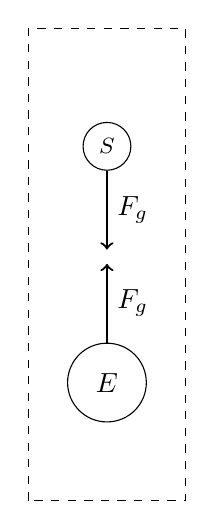
\begin{tikzpicture}
                \draw[dashed] (-1,-1.5) rectangle (1,4.5);
                %% earth and Satellite
                \node[draw,circle,minimum size=1cm] (E) at (0,0) {$E$};
                \node[draw,circle,minimum size=0.5cm,font=\footnotesize] (S) at (0,3) {$S$};
                %% vectors
                \draw[thick,->] (E.north) -- ++(90:1) node[pos=0.5,anchor=west] {$F_g$};
                \draw[thick,->] (S.south) -- ++(270:1) node[pos=0.5,anchor=west] {$F_g$};
            \end{tikzpicture}
        }
        \wrongchoice{
            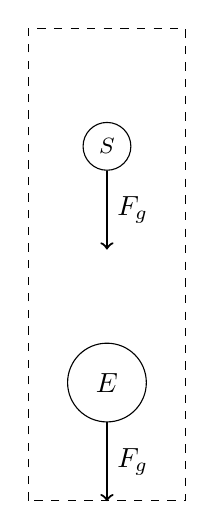
\begin{tikzpicture}
                \draw[dashed] (-1,-1.5) rectangle (1,4.5);
                %% earth and Satellite
                \node[draw,circle,minimum size=1cm] (E) at (0,0) {$E$};
                \node[draw,circle,minimum size=0.5cm,font=\footnotesize] (S) at (0,3) {$S$};
                %% vectors
                \draw[thick,->] (E.south) -- ++(270:1) node[pos=0.5,anchor=west] {$F_g$};
                \draw[thick,->] (S.south) -- ++(270:1) node[pos=0.5,anchor=west] {$F_g$};
            \end{tikzpicture}
        }
        \wrongchoice{
            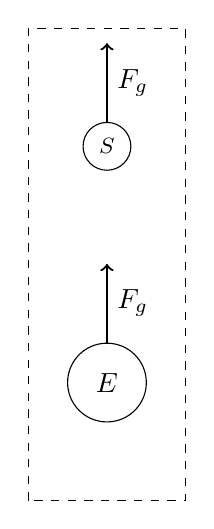
\begin{tikzpicture}
                \draw[dashed] (-1,-1.5) rectangle (1,4.5);
                %% earth and Satellite
                \node[draw,circle,minimum size=1cm] (E) at (0,0) {$E$};
                \node[draw,circle,minimum size=0.5cm,font=\footnotesize] (S) at (0,3) {$S$};
                %% vectors
                \draw[thick,->] (E.north) -- ++(90:1) node[pos=0.5,anchor=west] {$F_g$};
                \draw[thick,->] (S.north) -- ++(90:1) node[pos=0.5,anchor=west] {$F_g$};
            \end{tikzpicture}
        }
        \wrongchoice{
            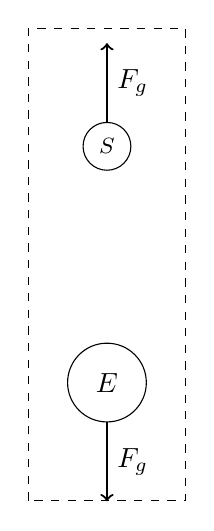
\begin{tikzpicture}
                \draw[dashed] (-1,-1.5) rectangle (1,4.5);
                %% earth and Satellite
                \node[draw,circle,minimum size=1cm] (E) at (0,0) {$E$};
                \node[draw,circle,minimum size=0.5cm,font=\footnotesize] (S) at (0,3) {$S$};
                %% vectors
                \draw[thick,->] (E.south) -- ++(270:1) node[pos=0.5,anchor=west] {$F_g$};
                \draw[thick,->] (S.north) -- ++(90:1) node[pos=0.5,anchor=west] {$F_g$};
            \end{tikzpicture}
        }
    \end{choices}
    \end{multicols}
\end{question}
}


%% Section Jan2008
%%--------------------
\element{nysed}{
\begin{question}{Jan2008-Q06}
    A \SI{60}{\kilo\gram} physics student would weigh \SI{1560}{\newton} on the surface of planet $X$.
    What is the magnitude of the acceleration due to gravity on the surface of planet $X$?
    \begin{multicols}{2}
    \begin{choices}
      \correctchoice{\SI{26}{\meter\per\second\squared}}
        \wrongchoice{\SI{9.8}{\meter\per\second\squared}}
        \wrongchoice{\SI{0.038}{\meter\per\second\squared}}
        \wrongchoice{\SI{6.1}{\meter\per\second\squared}}
    \end{choices}
    \end{multicols}
\end{question}
}


%% Section June2007
%%--------------------
\element{nysed}{
\begin{question}{June2007-Q10}
    Earth's mass is approximately \num{81} times the mass of the Moon.
    If Earth exerts a gravitational force of magnitude $F$ on the Moon,
        the magnitude of the gravitational force of the Moon on Earth is:
    \begin{multicols}{4}
    \begin{choices}
      \correctchoice{$F$}
        \wrongchoice{$\dfrac{F}{81}$}
        \wrongchoice{$9 F$}
        \wrongchoice{$81 F$}
    \end{choices}
    \end{multicols}
\end{question}
}

\element{nysed}{
\begin{question}{June2007-Q14}
    The diagram shows two bowling ball, $A$ and $B$,
        each having mass of \SI{7.00}{\kilo\gram}, placed \SI{2.0}{\meter} apart.
    \begin{center}
    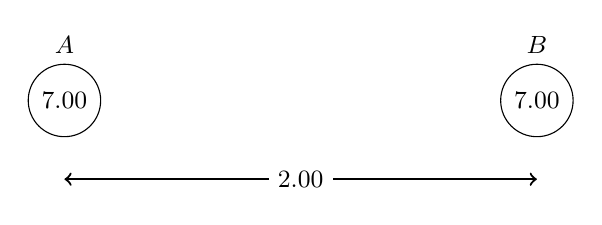
\begin{tikzpicture}[font=\small]
        %% Bowling ball A
        \node[draw,circle] (A) at (-3,0) {\SI{7.00}{\kilo\gram}};
        \node[anchor=south] at (A.north) {$A$};
        %% Bowling ball B
        \node[draw,circle] (B) at (+3,0) {\SI{7.00}{\kilo\gram}};
        \node[anchor=south] at (B.north) {$B$};
        %% distance
        \draw[<->,thick] (-3,-1) -- (3,-1) node[pos=0.5,anchor=center,fill=white] {\SI{2.00}{\meter}};
    \end{tikzpicture}
    \end{center}
    What is the magnitude of the gravitational force exerted by ball $A$ on ball $B$?
    \begin{multicols}{2}
    \begin{choices}
      \correctchoice{\SI{8.17e-10}{\newton}}
        \wrongchoice{\SI{1.17e-10}{\newton}}
        \wrongchoice{\SI{8.17e-9}{\newton}}
        \wrongchoice{\SI{1.63e-9}{\newton}}
    \end{choices}
    \end{multicols}
\end{question}
}


%% Section Jan2007
%%--------------------
\element{nysed}{
\begin{question}{Jan2007-Q10}
    As an astronaut travels from the surface of Earth to a position that is four times as far away from the center of Earth,
        the astronaut's:
    \begin{choices}
      \correctchoice{mass remains the same}
        \wrongchoice{mass decreases}
        \wrongchoice{weight increases}
        \wrongchoice{weight remains the same}
    \end{choices}
\end{question}
}


%% Section June2006
%%--------------------
\element{nysed}{
\begin{question}{June2006-Q11}
    Which diagram best represents the gravitational field lines surrounding Earth?
    \begin{multicols}{2}
    \begin{choices}
        \AMCboxDimensions{down=-1.2cm}
        \correctchoice{
            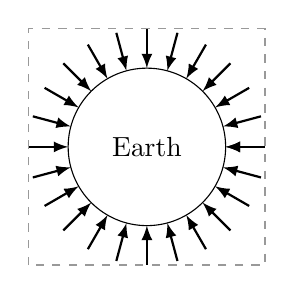
\begin{tikzpicture}
                \draw[dashed,white!60!black] (-1.5,-1.5) rectangle (1.5,1.5);
                %% Earth
                \node[anchor=center] at (0,0) {Earth};
                \draw (0,0) circle (1cm);
                %% field lines
                \foreach \x in {0,15,...,360} \draw[thick,latex-] (\x:1) -- (\x:1.5);
            \end{tikzpicture}
        }
        \wrongchoice{
            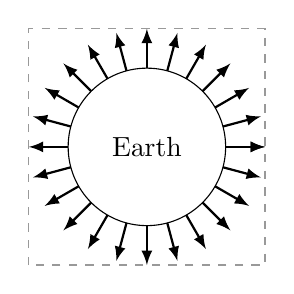
\begin{tikzpicture}
                \draw[dashed,white!60!black] (-1.5,-1.5) rectangle (1.5,1.5);
                %% Earth
                \node[anchor=center] at (0,0) {Earth};
                \draw (0,0) circle (1cm);
                %% field lines
                \foreach \x in {0,15,...,360} \draw[thick,-latex] (\x:1) -- (\x:1.5);
            \end{tikzpicture}
        }
        \wrongchoice{
            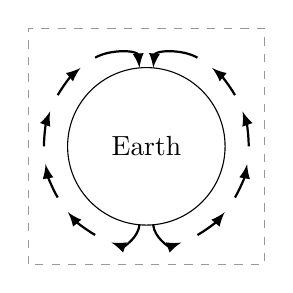
\begin{tikzpicture}
                \draw[dashed,white!60!black] (-1.5,-1.5) rectangle (1.5,1.5);
                %% Earth
                \node[anchor=center] at (0,0) {Earth};
                \draw (0,0) circle (1cm);
                %% field lines
                \draw[thick,-latex] (265:1) to[out=265,in=340,tension=0.7] (250:1.3);
                \draw[thick,-latex] (275:1) to[out=275,in=200,tension=0.7] (290:1.3);
                \foreach \x in {30,60,...,120} {
                    \draw[thick,-latex] ({270+\x}:1.3) arc({270+\x}:{270+\x+20}:1.3);
                    \draw[thick,-latex] ({270-\x}:1.3) arc({270-\x}:{270-\x-20}:1.3);
                }
                \draw[thick,-latex] (60:1.3) to[out=150,in=85] (85:1);
                \draw[thick,-latex] (120:1.3) to[out=30,in=95] (95:1);
            \end{tikzpicture}
        }
        \wrongchoice{
            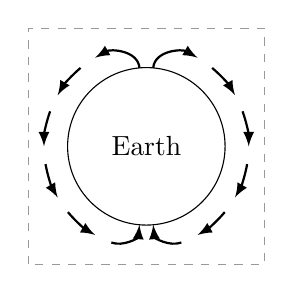
\begin{tikzpicture}
                \draw[dashed,white!60!black] (-1.5,-1.5) rectangle (1.5,1.5);
                %% Earth
                \node[anchor=center] at (0,0) {Earth};
                \draw (0,0) circle (1cm);
                %% field lines
                \draw[thick,latex-] (265:1) to[out=265,in=340,tension=0.7] (250:1.3);
                \draw[thick,latex-] (275:1) to[out=275,in=200,tension=0.7] (290:1.3);
                \foreach \x in {30,60,...,120} {
                    \draw[thick,latex-] ({270+\x}:1.3) arc({270+\x}:{270+\x+20}:1.3);
                    \draw[thick,latex-] ({270-\x}:1.3) arc({270-\x}:{270-\x-20}:1.3);
                }
                \draw[thick,latex-] (60:1.3) to[out=150,in=85,tension=0.7] (85:1);
                \draw[thick,latex-] (120:1.3) to[out=30,in=95,tension=0.7] (95:1);
            \end{tikzpicture}
        }
    \end{choices}
    \end{multicols}
\end{question}
}

\element{nysed}{
\begin{question}{June2006-Q37}
    A \SI{2.0}{\kilo\gram} object is falling freely near Earth's surface.
    What is the magnitude of the gravitational force that Earth exerts on the object?
    \begin{multicols}{2}
    \begin{choices}
      \correctchoice{\SI{20.}{\newton}}
        \wrongchoice{\SI{2.0}{\newton}}
        \wrongchoice{\SI{0.20}{\newton}}
        \wrongchoice{\SI{0.0}{\newton}}
    \end{choices}
    \end{multicols}
\end{question}
}


%% Section Jan2006
%%--------------------
\element{nysed}{
\begin{question}{Jan2006-Q06}
    A \SI{25.0}{\kilo\gram} space probe fell freely with an acceleration of \SI{2.00}{\meter\per\second\squared} just before it landed on a distant planet.
    What is the weight of the space probe on that planet?
    \begin{multicols}{2}
    \begin{choices}
        \wrongchoice{\SI{12.5}{\newton}}
      \correctchoice{\SI{50.0}{\newton}}
        \wrongchoice{\SI{25.0}{\newton}}
        \wrongchoice{\SI{250}{\newton}}
    \end{choices}
    \end{multicols}
\end{question}
}

\element{nysed}{
\begin{question}{Jan2006-Q13}
    The diagram below represents two satellites of equal mass, $A$ and $B$, in circular orbits around a planet.
    \begin{center}
    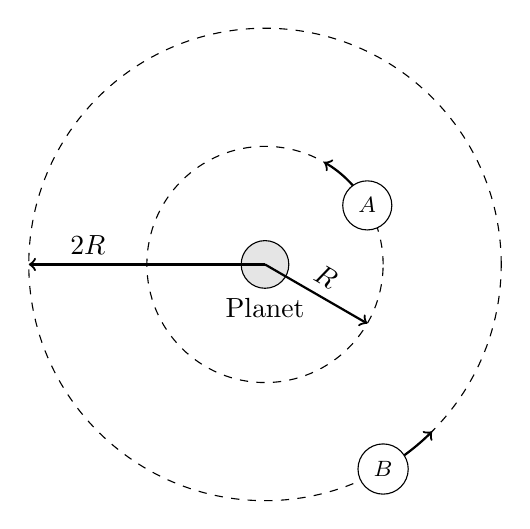
\begin{tikzpicture}
        %% Planet
        \draw[fill=white!90!black] (0,0) circle (2ex) node[anchor=north,yshift=-2ex] {Planet};
        %% R radius
        \draw[dashed] (0,0) circle (1.5);
        \draw[thick,->] (0,0) -- (330:1.5) node[pos=0.5,anchor=south,rotate=-30] {$R$};
        \draw[thick,->] (30:1.5) arc (30:60:1.5);
        \node[draw,circle,font=\footnotesize,fill=white] at (30:1.5) {$A$};
        %% 2R radius
        \draw[dashed] (0,0) circle (3);
        \draw[thick,->] (0,0) -- (180:3) node[pos=0.75,anchor=south] {$2R$};
        \draw[thick,->] (300:3) arc (300:315:3);
        \node[draw,circle,font=\footnotesize,fill=white] at (300:3) {$B$};
    \end{tikzpicture}
    \end{center}
    Compared to the magnitude of the gravitational force of attraction between satellite $A$ and the planet,
        the magnitude of the gravitational force of attraction between satellite $B$ and the planet is:
    \begin{choices}
      \correctchoice{one-fourth as great}
        \wrongchoice{four times as great}
        \wrongchoice{half as great}
        \wrongchoice{twice as great}
    \end{choices}
\end{question}
}


%% Section June2005
%%--------------------
\element{nysed}{
\begin{question}{June2005-Q09}
    A container of rocks with a mass of \SI{65.0}{\kilo\gram} is brought back from the moon's surface where the acceleration of gravity is \SI{1.62}{\meter\per\second}.
    What is the weight of the container of rocks on Earth's surface?
    \begin{multicols}{2}
    \begin{choices}
      \correctchoice{\SI{638}{\newton}}
        \wrongchoice{\SI{394}{\newton}}
        \wrongchoice{\SI{105}{\newton}}
        \wrongchoice{\SI{65.0}{\newton}}
    \end{choices}
    \end{multicols}
\end{question}
}

\element{nysed}{
\begin{question}{June2005-Q12}
    A satellite weighs \SI{200}{\newton} on the surface of Earth.
    What is its weight at a distance of one Earth radius above the surface of the Earth?
    \begin{multicols}{2}
    \begin{choices}
      \correctchoice{\SI{50}{\newton}}
        \wrongchoice{\SI{100}{\newton}}
        \wrongchoice{\SI{400}{\newton}}
        \wrongchoice{\SI{800}{\newton}}
    \end{choices}
    \end{multicols}
\end{question}
}


%% Section Jan2005
%%--------------------


%% Section June2004
%%--------------------
\element{nysed}{
\begin{question}{June2004-Q06}
    The acceleration due to gravity on the surface of planet $X$ is \SI{19.6}{\meter\per\second\squared}.
    If an object on the surface of this planet weighs \SI{980}{\newton},
        the mass of the object is:
    \begin{multicols}{2}
    \begin{choices}
      \correctchoice{\SI{50.0}{\kilo\gram}}
        \wrongchoice{\SI{490}{\kilo\gram}}
        \wrongchoice{\SI{908}{\kilo\gram}}
        \wrongchoice{\SI{100}{\kilo\gram}}
    \end{choices}
    \end{multicols}
\end{question}
}


%% Section Jan2004
%%--------------------
\newcommand{\JanTwentyFourQThirtySix}{
\begin{tabu}{X[c]X[3c]X[c]}
    \toprule
    Position & Distance from Earth's Center [\si{\meter}] & Weight [\si{\newton}] \\
    \midrule
    $A$  & \num{6.37e6} & \num{1.0e3} \\
    $B$  & \num{1.27e7} & \num{2.5e2} \\
    $C$  & \num{1.91e7} & \num{1.1e2} \\
    $D$  & \num{2.55e7} & \num{6.3e1} \\
    $E$  & \num{3.19e7} & \num{4.0e1} \\
    \bottomrule
\end{tabu}
}

\element{nysed}{
\begin{question}{Jan2004-Q36}
    The weight of an object was determined at five different distances from the center of Earth.
    The results are shown in the table below.
    Position $A$ represents results for the object at the surface of Earth.
    \begin{center}
        \JanTwentyFourQThirtySix
    \end{center}
    The approximate mass of the object is:
    \begin{multicols}{2}
    \begin{choices}
      \correctchoice{\SI{100}{\kilo\gram}}
        \wrongchoice{\SI{1000}{\kilo\gram}}
        \wrongchoice{\SI{0.01}{\kilo\gram}}
        \wrongchoice{\SI{10}{\kilo\gram}}
    \end{choices}
    \end{multicols}
\end{question}
}

\element{nysed}{
\begin{question}{Jan2004-Q37}
    The weight of an object was determined at five different distances from the center of Earth.
    The results are shown in the table below.
    Position $A$ represents results for the object at the surface of Earth.
    \begin{center}
        \JanTwentyFourQThirtySix
    \end{center}
    At what distance from the center of Earth is the weight of the object approximately \SI{28}{\newton}?
    \begin{multicols}{2}
    \begin{choices}
      \correctchoice{\SI{3.8e7}{\meter}}
        \wrongchoice{\SI{3.5e7}{\meter}}
        \wrongchoice{\SI{4.1e7}{\meter}}
        \wrongchoice{\SI{4.5e7}{\meter}}
    \end{choices}
    \end{multicols}
\end{question}
}

%% Section June2003
%%--------------------
\element{nysed}{
\begin{question}{June2003-Q09}
    An astronaut weighs \SI{8.00e2}{\newton} on the surface of Earth.
    What is the weight of the astronaut \SI{6.37e6}{\meter} above the surface of the Earth?
    \begin{multicols}{2}
    \begin{choices}
      \correctchoice{\SI{600}{\newton}}
        \wrongchoice{\SI{60}{\newton}}
        \wrongchoice{\SI{6}{\newton}}
        \wrongchoice{\SI{0}{\newton}}
    \end{choices}
    \end{multicols}
\end{question}
}


%% Section Jan2003
%%--------------------
\element{nysed}{
\begin{question}{Jan2003-Q06}
    The graph below represents the relationship between gravitational force and mass for objects near the surface of the Earth.
    \begin{center}
    \begin{tikzpicture}
        \begin{axis}[
            axis y line=left,
            axis x line=bottom,
            axis line style={->},
            ylabel={force},
            ytick=\empty,
            xlabel={mass},
            xtick=\empty,
            xmin=0,xmax=11,
            ymin=0,ymax=11,
            width=0.8\columnwidth,
            height=0.5\columnwidth,
        ]
        \addplot[line width=1pt,domain=0:10]{x};
        \end{axis}
    \end{tikzpicture}
    \end{center}
    The slope of the graph represents the:
    \begin{choices}
      \correctchoice{acceleration due to gravity}
        \wrongchoice{universal gravitational constant}
        \wrongchoice{momentum of objects}
        \wrongchoice{weight of objects}
    \end{choices}
\end{question}
}

\element{nysed}{
\begin{question}{Jan2003-Q14}
    An object weighs \SI{100}{\newton} on Earth's surface.
    When it is moved to a point one Earth radius above Earth's surface, it will weigh:
    \begin{multicols}{2}
    \begin{choices}
      \correctchoice{\SI{25.0}{\newton}}
        \wrongchoice{\SI{50.4}{\newton}}
        \wrongchoice{\SI{100}{\newton}}
        \wrongchoice{\SI{400}{\newton}}
    \end{choices}
    \end{multicols}
\end{question}
}


%% Section Aug2002
%%--------------------
\element{nysed}{
\begin{question}{Aug2002-Q26}
    The centers of two \SI{15.0}{\kilo\gram} spheres are separated by \SI{3.00}{\meter}.
    The magnitude of the gravitational force between the two spheres is approximately:
    \begin{multicols}{2}
    \begin{choices}
        \wrongchoice{\SI{1.11e-10}{\newton}}
        \wrongchoice{\SI{3.34e-10}{\newton}}
      \correctchoice{\SI{1.67e-9}{\newton}}
        \wrongchoice{\SI{5.00e-9}{\newton}}
    \end{choices}
    \end{multicols}
\end{question}
}


%% Section June2002
%%--------------------


%% Section Jan2002
%%--------------------
\element{nysed}{
\begin{question}{Jan2002-Q10}
    When a satellite is a distance $R$ from the center of Earth, the force due to gravity on the satellite is $F$.
    What is the force due to gravity on the satellite when its distance from the center of Earth is $3R$?
    \begin{multicols}{4}
    \begin{choices}
      \correctchoice{$\dfrac{F}{9}$}
        \wrongchoice{$\dfrac{F}{3}$}
        \wrongchoice{$F$}
        \wrongchoice{$9F$}
    \end{choices}
    \end{multicols}
\end{question}
}

\element{nysed}{
\begin{question}{Jan2002-Q15}
    Which graph best represents the relationship between acceleration due to gravity and mass for objects near the surface of Earth?
    [Neglect air resistance.]
    \begin{multicols}{2}
    \begin{choices}
        \AMCboxDimensions{down=-2.5em}
        \correctchoice{
            \begin{tikzpicture}
                \begin{axis}[
                    axis y line=left,
                    axis x line=bottom,
                    axis line style={->},
                    xlabel={mass},
                    xtick=\empty,
                    ylabel={acceleration},
                    ytick=\empty,
                    xmin=0,xmax=11,
                    ymin=0,ymax=11,
                    width=\columnwidth,
                    very thin,
                ]
                \addplot[line width=1pt,domain=0:10]{8};
                \end{axis}
            \end{tikzpicture}
        }
        \wrongchoice{
            \begin{tikzpicture}
                \begin{axis}[
                    axis y line=left,
                    axis x line=middle,
                    axis line style={->},
                    xlabel={mass},
                    xtick=\empty,
                    ylabel={acceleration},
                    ytick=\empty,
                    xmin=0,xmax=11,
                    ymin=0,ymax=11,
                    width=\columnwidth,
                    very thin,
                ]
                \addplot[line width=1pt,domain=0:10]{x};
                \end{axis}
            \end{tikzpicture}
        }
        \wrongchoice{
            \begin{tikzpicture}
                \begin{axis}[
                    axis y line=left,
                    axis x line=bottom,
                    axis line style={->},
                    xlabel={mass},
                    xtick=\empty,
                    ylabel={acceleration},
                    ytick=\empty,
                    xmin=0,xmax=11,
                    ymin=0,ymax=11,
                    width=\columnwidth,
                    very thin,
                ]
                \addplot[line width=1pt,domain=0:10]{10/x};
                \end{axis}
            \end{tikzpicture}
        }
        \wrongchoice{
            \begin{tikzpicture}
                \begin{axis}[
                    axis y line=left,
                    axis x line=bottom,
                    axis line style={->},
                    xlabel={mass},
                    xtick=\empty,
                    ylabel={acceleration},
                    ytick=\empty,
                    xmin=0,xmax=11,
                    ymin=0,ymax=11,
                    width=\columnwidth,
                    very thin,
                ]
                \addplot[line width=1pt,domain=0:10]{0.1*x*x};
                \end{axis}
            \end{tikzpicture}
        }
    \end{choices}
    \end{multicols}
\end{question}
}

\element{nysed}{
\begin{question}{Jan2002-Q61}
    The diagram below represents the path of Earth around the Sun.
    \begin{center}
    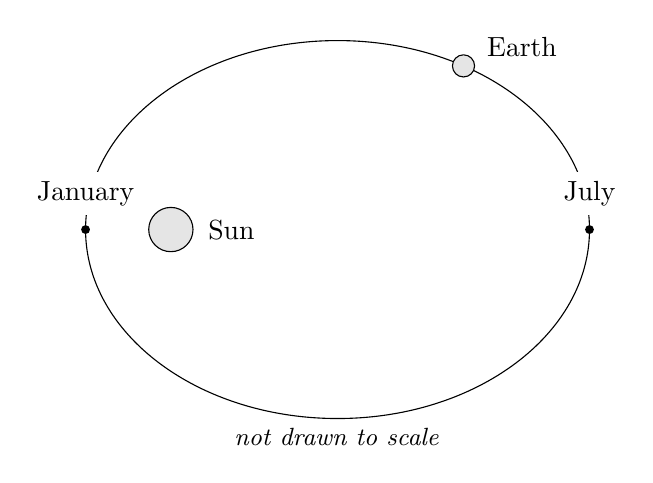
\begin{tikzpicture}[scale=0.8]
        \def\a{4}
        \def\b{3}
        %% orbit
        \draw (0,0) circle (\a{} and \b);
        %% Sun and Earth
        \draw[fill=white!90!black] ({-sqrt(\a*\a-\b*\b)},0) circle (1em) node[anchor=west,xshift=1em] {Sun};
        \draw[fill=white!90!black] ({\a*cos(60)},{\b*sin(60)}) circle (0.5em) node[anchor=south west,xshift=0.5em] {Earth};
        %% January and July
        \foreach \x/\y in {180/January,0/July}
            \fill ({\a*cos(\x)},{\b*sin(\x)}) circle (2pt) node[anchor=south,yshift=5pt,fill=white] {\y};
        \node[anchor=north,font=\small] at (0,-3) {\emph{not drawn to scale}};
    \end{tikzpicture}
    \end{center}
    As Earth travels in its orbit from its January position to its July position,
        the potential energy of Earth:
    \begin{choices}
        \wrongchoice{decreases and its kinetic energy decreases}
        \wrongchoice{decreases and its kinetic energy increases}
      \correctchoice{increases and its kinetic energy decreases}
        \wrongchoice{increases and its kinetic energy increases}
    \end{choices}
\end{question}
}

\element{nysed}{
\begin{question}{Jan2002-Q64}
    What is the period of orbit of a communications satellite in geosynchronous orbit about Earth?
    \begin{multicols}{2}
    \begin{choices}
        \wrongchoice{\num{1} year}
      \correctchoice{\num{24} hours}
        \wrongchoice{\num{12} hours}
        \wrongchoice{\num{60} minutes}
    \end{choices}
    \end{multicols}
\end{question}
}

\element{nysed}{
\begin{question}{Jan2002-Q65}
    The table below gives information about the Moon and a satellite orbiting Earth.
    \begin{center}\small
    \begin{tabu}{rcX[l]}
        $R_m$ & = & mean radius of orbit of the Moon around Earth \\ 
        $R_s$ & = & mean radius of orbit of satellite around Earth \\ 
        $T_m$ & = & period of orbit of the Moon around Earth \\ 
        $T_s$ & = & period of orbit of satellite around Earth \\ 
    \end{tabu}
    \end{center}
    Which equation correctly relates these quantities?
    \begin{multicols}{2}
    \begin{choices}
        \wrongchoice{$R_m T_m = R_s T_s$}
        \wrongchoice{$R_m T_s = R_s T_m$}
        \wrongchoice{$\dfrac{R_m^2}{T_m} = \dfrac{R_s^2}{T_s}$}
      \correctchoice{$\dfrac{R_m^3}{T_m^2} = \dfrac{R_s^3}{T_s^2}$}
    \end{choices}
    \end{multicols}
\end{question}
}


%% Section June2001
%%--------------------
\element{nysed}{
\begin{question}{June2001-Q04}
    An astronaut weighs \SI{500}{\newton} on Earth and \SI{25}{\newton} on asteroid $X$.
    The acceleration due to gravity on asteroid $X$ is approximately:
    \begin{multicols}{2}
    \begin{choices}
        \wrongchoice{\SI{1}{\meter\per\second\squared}}
        \wrongchoice{\SI{2}{\meter\per\second\squared}}
        \wrongchoice{\SI{0.2}{\meter\per\second\squared}}
      \correctchoice{\SI{0.5}{\meter\per\second\squared}}
    \end{choices}
    \end{multicols}
\end{question}
}

\element{nysed}{
\begin{question}{June2001-Q54}
    The radius of Mars is approximately one-half the radius of Earth, and the mass of Mars is approximately one-tenth the mass of Earth.
    Compared to the acceleration due to gravity on the surface of Earth, the acceleration due to gravity on the surface of Mars is:
    \begin{multicols}{3}
    \begin{choices}
      \correctchoice{smaller}
        \wrongchoice{larger}
        \wrongchoice{the same}
    \end{choices}
    \end{multicols}
\end{question}
}

\element{nysed}{
\begin{question}{June2001-Q63}
    The diagram below shows the elliptical orbit of a comet around the sun.
    The comet's closest approach to the Sun is at point $A$.
    \begin{center}
    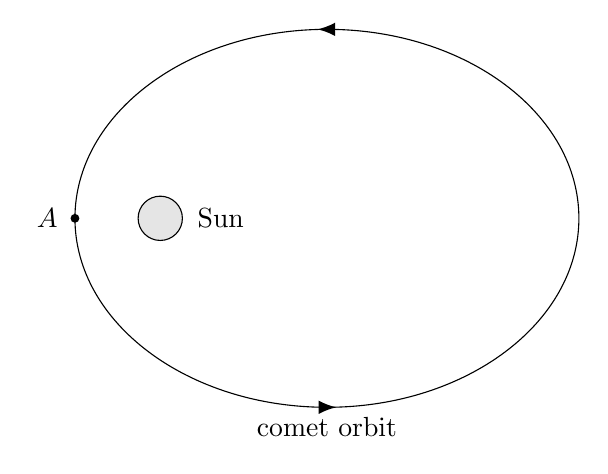
\begin{tikzpicture}[scale=0.8]
        \def\a{4}
        \def\b{3}
        %% orbit
        \draw (0,0) circle (\a{} and \b);
        \draw[very thick,-latex] (0,-\b) -- ++(0:1ex);
        \draw[very thick,-latex] (0,+\b) -- ++(180:1ex);
        \node[anchor=north] at (0,-\b) {comet orbit};
        %% Sun
        \draw[fill=white!90!black] ({-sqrt(\a*\a-\b*\b)},0) circle (1em) node[anchor=west,xshift=1em] {Sun};
        %% labels
        \foreach \x/\y in {180/A}
            \fill ({\a*cos(\x)},{\b*sin(\x)}) circle (2pt) node[anchor=center,shift={(\x:1em)}] {$\y$};
    \end{tikzpicture}
    \end{center}
    Which statement best describes the comet's energy as it passes through point $A$?
    \begin{choices}
        \wrongchoice{Its kinetic energy is at a minimum and its potential energy is at a minimum.}
        \wrongchoice{Its kinetic energy is at a minimum and its potential energy is at a maximum.}
      \correctchoice{Its kinetic energy is at a maximum and its potential energy is at a minimum.}
        \wrongchoice{Its kinetic energy is at a maximum and its potential energy is at a maximum.}
    \end{choices}
\end{question}
}

\element{nysed}{
\begin{question}{June2001-Q64}
    %The chart below gives the mass and orbital period of each of four satellites, $A$, $B$, $C$, and $D$, orbiting Earth in circular paths.
    %% NOTE: changed option formatting
    The mass and orbital period for four satellites is provided.
    Which satellite is closest to Earth?
    \begin{center}
    \begin{tabu}{cX[c]X[2c]}
        \toprule
        \makebox[1.5em][c]{\textnumero}
            & Mass [\si{\kilo\gram}] & Orbital Period [\si{\hour}] \\
        \bottomrule
    \end{tabu}
    \end{center}
    \begin{choices}
        \wrongchoice{\begin{tabu}{X[c]X[2c]} 500 & 4 \\ \end{tabu}}
      \correctchoice{\begin{tabu}{X[c]X[2c]} 500 & 2 \\ \end{tabu}}
        \wrongchoice{\begin{tabu}{X[c]X[2c]} 100 & 6 \\ \end{tabu}}
        \wrongchoice{\begin{tabu}{X[c]X[2c]} 100 & 3 \\ \end{tabu}}
    \end{choices}
\end{question}
}

\element{nysed}{
\begin{question}{June2001-Q65}
    The Moon's orbit is \emph{not} classified as geosynchronous because:
    \begin{choices}
      \correctchoice{the Moon's position over Earth's surface varies with time}
        \wrongchoice{the Moon's mass is very large compared to the mass of all other Earth satellites}
        \wrongchoice{the Moon is a natural satellite, rather than an artificial one}
        \wrongchoice{the Moons always has the same half of its surface facing Earth}
    \end{choices}
\end{question}
}


%% Section Jan2001
%%--------------------
\element{nysed}{
\begin{question}{Jan2001-Q09}
    What is the magnitude of the gravitational force between two \SI{5.0}{\kilo\gram} masses separated by a distance of \SI{5.0}{\meter}?
    \begin{multicols}{2}
    \begin{choices}
      \correctchoice{\SI{6.7e-11}{\newton}}
        \wrongchoice{\SI[retain-zero-exponent]{5.0e0}{\newton}}
        \wrongchoice{\SI{3.3e-10}{\newton}}
        \wrongchoice{\SI{1.3e-10}{\newton}}
    \end{choices}
    \end{multicols}
\end{question}
}

\element{nysed}{
\begin{question}{Jan2001-Q60}
    The diagram below shows four different locations of a satellite in its elliptical orbit about Earth.
    \begin{center}
    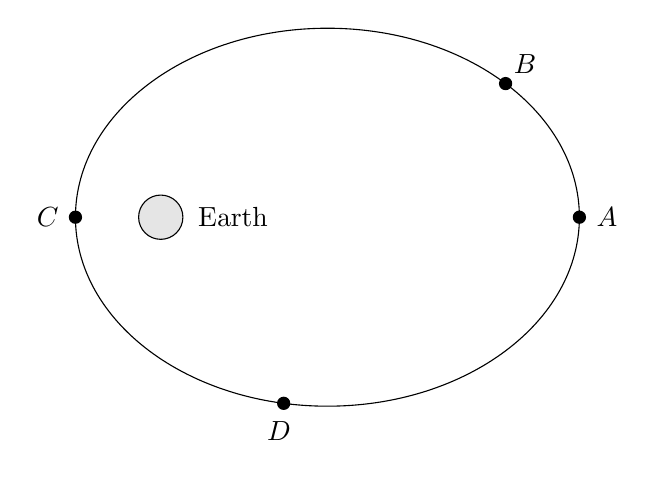
\begin{tikzpicture}[scale=0.8]
        \def\a{4}
        \def\b{3}
        %% orbit
        \draw (0,0) circle (\a{} and \b);
        %% Earth
        \draw[fill=white!90!black] ({-sqrt(\a*\a-\b*\b)},0) circle (1em) node[anchor=west,xshift=1em] {Earth};
        %% labels
        \foreach \x/\y in {0/A,45/B,180/C,260/D}
            \fill ({\a*cos(\x)},{\b*sin(\x)}) circle (3pt) node[anchor=center,shift={(\x:1em)}] {$\y$};
    \end{tikzpicture}
    \end{center}
    At which location is the magnitude of the satellite's velocity greatest?
    \begin{multicols}{4}
    \begin{choices}[o]
        \wrongchoice{$A$}
        \wrongchoice{$B$}
      \correctchoice{$C$}
        \wrongchoice{$D$}
    \end{choices}
    \end{multicols}
\end{question}
}

\element{nysed}{
\begin{question}{Jan2001-Q61}
    Which statement is consistent with Kepler's laws of planetary motion?
    \begin{choices}
        \wrongchoice{The planets move at a constant speed around the Sun}
        \wrongchoice{The speed of a planet is directly proportional to the radius of the path of motion}
        \wrongchoice{The more massive the planet, the slower the planet moves around the sun}
      \correctchoice{An imaginary line from a planet to the Sun sweeps out equal areas in equal time intervals}
    \end{choices}
\end{question}
}

\element{nysed}{
\begin{question}{Jan2001-Q64}
    The table below gives the mean radius of orbit and orbital period for two moons of a planet.
    \begin{center}
    \begin{tabu}{X[c]X[c]X[c]}
        \toprule
        Moon & Mean Radius of Orbit & Orbital Period \\
        \midrule
        $A$ & $R$  & $T$ \\
        $B$ & $4R$ & $8T$ \\
        \bottomrule
    \end{tabu}
    \end{center}
    Compared to the ratio of the orbital radius cubed to the period squared for Moon $A$, the ratio:
    \begin{multicols}{3}
    \begin{choices}
        \wrongchoice{less}
        \wrongchoice{greater}
      \correctchoice{the same}
    \end{choices}
    \end{multicols}
\end{question}
}

\element{nysed}{
\begin{question}{Jan2001-Q65}
    A satellite is in geosynchronous orbit.
    Compared to Earth's period of rotation,
        the satellite's period of revolution is:
    \begin{multicols}{3}
    \begin{choices}
        \wrongchoice{less}
        \wrongchoice{greater}
      \correctchoice{the same}
    \end{choices}
    \end{multicols}
\end{question}
}


%% Section June2000
%%--------------------
\element{nysed}{
\begin{question}{June2000-Q19}
    The gravitational force of attraction between two objects would be increased by
    \begin{choices}
      \correctchoice{doubling the mass of both objects, only}
        \wrongchoice{doubling the distance between the objects, only}
        \wrongchoice{doubling the mass of both objects and doubling the distance between the objects}
        \wrongchoice{doubling the mass of one object and doubling the distance between the objects}
    \end{choices}
\end{question}
}

\newcommand{\JuneTwoThousandQSixtyOne}{
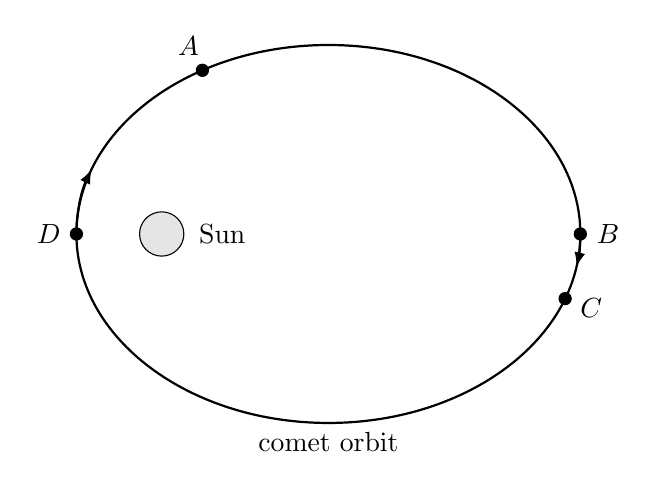
\begin{tikzpicture}[scale=0.8]
    \def\a{4}
    \def\b{3}
    %% orbit
    \draw[thick] (0,0) circle (\a{} and \b);
    \draw[thick,-latex] (-\a,0) arc (180:160:\a{} and \b);
    \draw[thick,-latex] (+\a,0) arc (360:350:\a{} and \b);
    \node[anchor=north] at (0,-\b) {comet orbit};
    %% Sun
    \draw[fill=white!90!black] ({-sqrt(\a*\a-\b*\b)},0) circle (1em) node[anchor=west,xshift=1em] {Sun};
    %% labels
    \foreach \x/\y in {120/A,0/B,340/C,180/D}
        \fill ({\a*cos(\x)},{\b*sin(\x)}) circle (3pt) node[anchor=center,shift={(\x:1em)}] {$\y$};
\end{tikzpicture}
}

\element{nysed}{
\begin{question}{June2000-Q61}
    The diagram below represents the orbit of a comet about the sun.
    %% NOTE: near dup of Jan2001-Q60
    \begin{center}
        \JuneTwoThousandQSixtyOne
    \end{center}
    At which position in its orbit is the comet's speed greatest?
    \begin{multicols}{4}
    \begin{choices}[o]
        \wrongchoice{$A$}
        \wrongchoice{$B$}
        \wrongchoice{$C$}
      \correctchoice{$D$}
    \end{choices}
    \end{multicols}
\end{question}
}

\element{nysed}{
\begin{question}{June2000-Q62}
    The diagram below represents the orbit of a comet about the sun.
    \begin{center}
        \JuneTwoThousandQSixtyOne
    \end{center}
    As the comet moves from point $A$ to point $B$,
        its potential energy:
    \begin{choices}
        \wrongchoice{decreases}
      \correctchoice{increases}
        \wrongchoice{remains the same}
    \end{choices}
\end{question}
}

\element{nysed}{
\begin{question}{June2000-Q63}
    The diagram below shows a satellite of mass $m$ orbiting Earth in a circular path of radius $R$.
    \begin{center}
    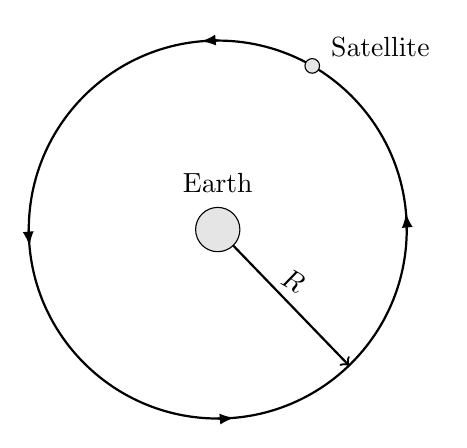
\begin{tikzpicture}[scale=0.8]
        %% orbit
        \draw[thick] (0,0) circle (3);
        \foreach \x in {0,90,180,270}
            \draw[thick,-latex] (\x:3) arc (\x:{\x+5}:3);
        \draw[thick,->] (0,0) -- (314:3) node[pos=0.5,anchor=south,rotate=-30] {$R$};
        %% Earth
        \draw[fill=white!90!black] (0,0) circle (1em) node[anchor=south,yshift=1em] {Earth};
        %% Satelite
        \draw[fill=white!90!black] (60:3) circle (0.33em) node[anchor=south west,xshift=0.33em] {Satellite};
    \end{tikzpicture}
    \end{center}
    If centripetal force $F_c$ is acting on the satellite,
        its speed is equal to:
    \begin{multicols}{2}
    \begin{choices}
      \correctchoice{$\sqrt{\dfrac{F_c R}{m}}$}
        \wrongchoice{$\dfrac{F_c R}{m}$}
        \wrongchoice{$\sqrt{\dfrac{F_c m}{R}}$}
        \wrongchoice{$F_c mR$}
    \end{choices}
    \end{multicols}
\end{question}
}

\element{nysed}{
\begin{question}{June2000-Q65}
    The symbols below are terms for Earth orbiting the sun and a comet orbiting the Sun.
    \begin{center}
    \begin{tabu}{rcX[l]}
        $R_e$ & = & the mean radius of Earth's orbit \\
        $T_e$ & = & the period of Earth's orbit \\
        $R_c$ & = & the mean radius the comet's orbit \\
        $T_c$ & = & the period of the comet's orbit \\
    \end{tabu}
    \end{center}
    Compared to the values of $\dfrac{R_e^3}{T_e^2}$ the value of $\dfrac{R_c^3}{T_c^2}$ is:
    %% Kepler's third law (harmonic law)
    %% P^2 / a^3 is constant
    \begin{multicols}{3}
    \begin{choices}
        \wrongchoice{smaller}
        \wrongchoice{larger}
      \correctchoice{the same}
    \end{choices}
    \end{multicols}
\end{question}
}


%% Section June1999
%%--------------------
\element{nysed}{
\begin{question}{June1999-Q13}
    The graph below shows the relationship between weight and mass for a series of objects on the Moon.
    \begin{center}
    \begin{tikzpicture}
        \begin{axis}[
            axis y line=left,
            axis x line=bottom,
            axis line style={->},
            title={Weight vs. Mass on the Moon},
            xlabel={Mass},
            x unit=\si{\kilo\gram},
            xtick={0,5,10,15,20},
            ylabel={Weight},
            y unit=\si{\newton},
            ytick={0,8,16,24,32},
            grid=major,
            xmin=0,xmax=21,
            ymin=0,ymax=33,
            width=0.8\columnwidth,
            height=0.5\columnwidth,
        ]
        \addplot[line width=1pt,domain=0:20]{1.6*x};
        \end{axis}
    \end{tikzpicture}
    \end{center}
    The acceleration due to gravity on the Moon is approximately:
    \begin{multicols}{2}
    \begin{choices}
        \wrongchoice{\SI{0.63}{\meter\per\second\squared}}
      \correctchoice{\SI{1.6}{\meter\per\second\squared}}
        \wrongchoice{\SI{9.8}{\meter\per\second\squared}}
        \wrongchoice{\SI{32}{\meter\per\second\squared}}
    \end{choices}
    \end{multicols}
\end{question}
}

\element{nysed}{
\begin{question}{June1999-Q16}
    Which graph best represents the relationship between the mass of a satellite launched from Earth and the satellite's distance away from Earth?
    \begin{multicols}{2}
    \begin{choices}
        \AMCboxDimensions{down=-2.5em}
        \correctchoice{
            \begin{tikzpicture}
                \begin{axis}[
                    axis y line=left,
                    axis x line=middle,
                    axis line style={->},
                    xlabel={mass},
                    xtick=\empty,
                    ylabel={distance},
                    ytick=\empty,
                    xmin=0,xmax=11,
                    ymin=0,ymax=11,
                    width=\columnwidth,
                    very thin,
                ]
                \addplot[line width=1pt,domain=0:10]{8};
                \end{axis}
            \end{tikzpicture}
        }
        \wrongchoice{
            \begin{tikzpicture}
                \begin{axis}[
                    axis y line=left,
                    axis x line=bottom,
                    axis line style={->},
                    xlabel={mass},
                    xtick=\empty,
                    ylabel={distance},
                    ytick=\empty,
                    xmin=0,xmax=11,
                    ymin=0,ymax=11,
                    width=\columnwidth,
                    very thin,
                ]
                \addplot[line width=1pt,domain=0:10]{x};
                \end{axis}
            \end{tikzpicture}
        }
        \wrongchoice{
            \begin{tikzpicture}
                \begin{axis}[
                    axis y line=left,
                    axis x line=bottom,
                    axis line style={->},
                    xlabel={mass},
                    xtick=\empty,
                    ylabel={distance},
                    ytick=\empty,
                    xmin=0,xmax=11,
                    ymin=0,ymax=11,
                    width=\columnwidth,
                    very thin,
                ]
                \addplot[line width=1pt,domain=0:10]{10-x};
                \end{axis}
            \end{tikzpicture}
        }
        \wrongchoice{
            \begin{tikzpicture}
                \begin{axis}[
                    axis y line=left,
                    axis x line=bottom,
                    axis line style={->},
                    xlabel={mass},
                    xtick=\empty,
                    ylabel={distance},
                    ytick=\empty,
                    xmin=0,xmax=11,
                    ymin=0,ymax=11,
                    width=\columnwidth,
                    very thin,
                ]
                \addplot[line width=1pt,domain=0:10]{10/x};
                \end{axis}
            \end{tikzpicture}
        }
    \end{choices}
    \end{multicols}
\end{question}
}

\element{nysed}{
\begin{question}{June1999-Q59}
    The diagram below shows the elliptical orbit of a comet around the sun.
    \begin{center}
    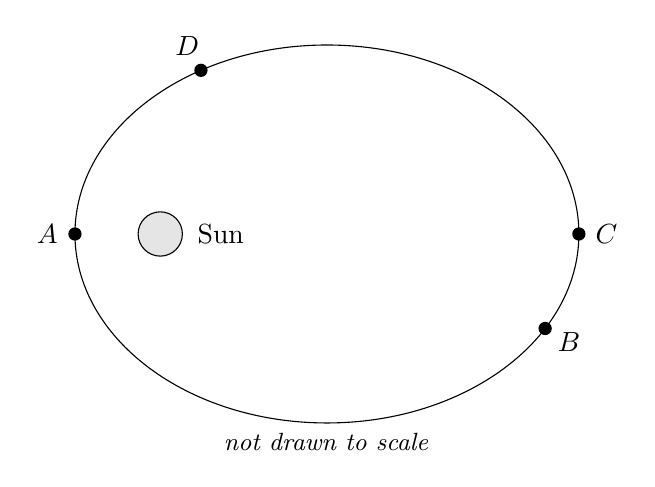
\begin{tikzpicture}[scale=0.8]
        \def\a{4}
        \def\b{3}
        %% orbit
        \draw (0,0) circle (\a{} and \b);
        %% Sun
        \draw[fill=white!90!black] ({-sqrt(\a*\a-\b*\b)},0) circle (1em) node[anchor=west,xshift=1em] {Sun};
        %% labels
        \foreach \x/\y in {180/A,330/B,0/C,120/D}
            \fill ({\a*cos(\x)},{\b*sin(\x)}) circle (3pt) node[anchor=center,shift={(\x:1em)}] {$\y$};
        \node[anchor=north,font=\small] at (0,-\b) {\emph{not drawn to scale}};
    \end{tikzpicture}
    \end{center}
    The magnitude of the centripetal acceleration of the comet is greatest at point:
    \begin{multicols}{4}
    \begin{choices}[o]
      \correctchoice{$A$}
        \wrongchoice{$B$}
        \wrongchoice{$C$}
        \wrongchoice{$D$}
    \end{choices}
    \end{multicols}
\end{question}
}

\element{nysed}{
\begin{question}{June1999-Q60}
    A communications satellite in geosynchronous orbit around Earth remains over the same location on Earth.
    The satellite's period of revolution about Earth is closest to:
    \begin{multicols}{2}
    \begin{choices}
        \wrongchoice{\num{1} hour}
      \correctchoice{\num{1} day}
        \wrongchoice{\num{1} month}
        \wrongchoice{\num{1} year}
    \end{choices}
    \end{multicols}
\end{question}
}

\element{nysed}{
\begin{question}{June1999-Q61}
    Which orbit diagram best represents the relative motion of the planet Saturn and the Sun?
    [Points $F_1$ and $F_2$ represent foci. Images are not drawn to scale.]
    \begin{multicols}{2}
    \begin{choices}
        \AMCboxDimensions{down=-2em}
      \correctchoice{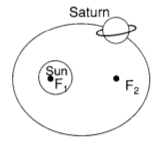
\includegraphics[keepaspectratio,scale=0.75]{June1999-Q61-A}}
        \wrongchoice{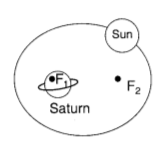
\includegraphics[keepaspectratio,scale=0.75]{June1999-Q61-B}}
        \wrongchoice{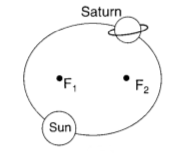
\includegraphics[keepaspectratio,scale=0.75]{June1999-Q61-C}}
        \wrongchoice{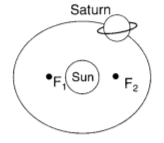
\includegraphics[keepaspectratio,scale=0.75]{June1999-Q61-D}}
    \end{choices}
    \end{multicols}
\end{question}
}


%% Section June1998
%%--------------------
\element{nysed}{
\begin{question}{June1998-Q10}
    What is the magnitude of the gravitational force between an electron and a proton separated by a distance of \SI{1.0e-10}{\meter}?
    \begin{multicols}{2}
    \begin{choices}
      \correctchoice{\SI{1.0e-47}{\newton}}
        \wrongchoice{\SI{1.5e-46}{\newton}}
        \wrongchoice{\SI{1.0e-37}{\newton}}
        \wrongchoice{\SI{1.5e-36}{\newton}}
    \end{choices}
    \end{multicols}
\end{question}
}

\element{nysed}{
\begin{question}{June1998-Q11}
    On the surface of planet $X$, the acceleration due to gravity is \SI{16}{\meter\per\second\squared}.
    What is the weight of a \SI{6.0}{\kilo\gram} mass located on the surface of planet $X$?
    \begin{multicols}{2}
    \begin{choices}
        \wrongchoice{\SI{2.7}{\newton}}
        \wrongchoice{\SI{59}{\newton}}
      \correctchoice{\SI{96}{\newton}}
        \wrongchoice{\SI{940}{\newton}}
    \end{choices}
    \end{multicols}
\end{question}
}

\newcommand{\JuneNineteenNinetyEightQSixtyThree}{
\begin{tikzpicture}[scale=0.95]
    %% A, B, C, D
    \def\a{4}
    \def\b{3}
    \draw (0,0) circle (\a{} and \b);
    \foreach \x/\y in {355/A,5/B,155/C,204/D}
        \fill ({\a*cos(\x)},{\b*sin(\x)}) circle (2pt) node[anchor=center,shift={(\x:1em)}] {$\y$};
    %% Planet P
    \foreach \x/\y in {300/P}
        \node[anchor=center,fill=white,draw,circle] at ({\a*cos(\x)},{\b*sin(\x)})  {$\y$};
    %% fill areas
    \draw[pattern=north east lines] ({-sqrt(\a*\a-\b*\b)},0) -- ({\a*cos(155)},{\b*sin(155)}) arc(155:204:\a{} and \b) -- cycle;
    \draw[pattern=north east lines] ({-sqrt(\a*\a-\b*\b)},0) -- ({\a*cos(5)},{\b*sin(5)}) arc(5:-5:\a{} and \b) -- cycle;
    %% Sun
    \node[anchor=center,draw,circle,fill=white] at ({-sqrt(\a*\a-\b*\b)},0) {$S$};
\end{tikzpicture}
}

\element{nysed}{
\begin{question}{June1998-Q63}
    A planet $P$, moves around the Sun, $S$, in an elliptical orbit.
    The amount of time required for the planet to travel from point $A$ to point $B$ is equal to the amount of time required to travel from point $C$ to point $D$.
    \begin{center}
        \JuneNineteenNinetyEightQSixtyThree
    \end{center}
    As the planet moves from point $B$ to point $C$, how does its kinetic energy and potential energy change?
    \begin{choices}
        \wrongchoice{Its kinetic energy decreases, and its potential energy decreases.}
        \wrongchoice{Its kinetic energy decreases, and its potential energy increases.}
      \correctchoice{Its kinetic energy increases, and its potential energy decreases.}
        \wrongchoice{Its kinetic energy increases, and its potential energy increases.}
    \end{choices}
\end{question}
}

\element{nysed}{
\begin{question}{June1998-Q64}
    A planet $P$, moves around the Sun, $S$, in an elliptical orbit.
    The amount of time required for the planet to travel from point $A$ to point $B$ is equal to the amount of time required to travel from point $C$ to point $D$.
    \begin{center}
        \JuneNineteenNinetyEightQSixtyThree
    \end{center}
    Compared to the area of region $ABS$, the area of region $CDS$ is:
    \begin{multicols}{3}
    \begin{choices}
        \wrongchoice{smaller}
        \wrongchoice{larger}
      \correctchoice{the same}
    \end{choices}
    \end{multicols}
\end{question}
}

\element{nysed}{
\begin{question}{June1998-Q65}
    The diagram below shows four planets, $A$, $B$, $C$, and $D$, orbiting a star.
    \begin{center}
    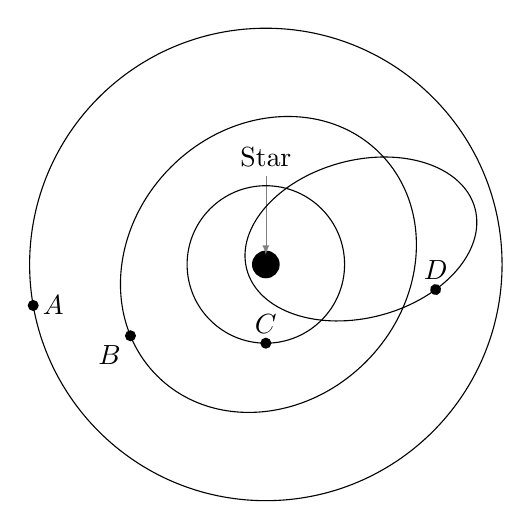
\begin{tikzpicture}
        %% star
        \fill (0,0) circle (5pt) node[pin={[pin edge={latex-},pin distance=1cm]90:Star}] {};
        %% orbit a
        \draw (0,0) circle (3cm);
        \fill (190:3) circle (2pt) node[anchor=west] {$A$};
        %% orbit b
        \draw[xshift=0.9375,rotate=45] (0,0) circle (2cm and 1.75cm);
        \fill[xshift=0.9375,rotate=45] ({2.00*cos(160)},{1.75*sin(160)}) circle (2pt) node[anchor=north east] {$B$};
        %% orbit c
        \draw (0,0) circle (1cm);
        \fill (270:1) circle (2pt) node[anchor=south] {$C$};
        %% orbit d
        \draw[rotate=15,xshift=1.25cm] (0,0) circle (1.5cm and 1.0cm);
        \fill[rotate=15,xshift=1.25cm] ({1.5*cos(300)},{1.0*sin(300)}) circle (2pt) node[anchor=south] {$D$};
    \end{tikzpicture}
    \end{center}
    Which planet has the greatest orbital period?
    %% Kepler's Law
    %% T^2 / R^3 = constant
    \begin{multicols}{4}
    \begin{choices}[o]
      \correctchoice{$A$}
        \wrongchoice{$B$}
        \wrongchoice{$C$}
        \wrongchoice{$D$}
    \end{choices}
    \end{multicols}
\end{question}
}


%% Section June1997
%%--------------------
\element{nysed}{
\begin{question}{June1997-Q11}
    The graph below shows the weight of three objects on planet $X$ as a function of their mass.
    \begin{center}
    \begin{tikzpicture}
        \begin{axis}[
            axis y line=left,
            axis x line=bottom,
            axis line style={->},
            ylabel={Weight},
            y unit=\si{\newton},
            ytick={0,100,200,300,400,500},
            xlabel={Mass},
            x unit=\si{\kilo\gram},
            xtick={0,25,50,75},
            xmin=0,xmax=75,
            ymin=0,ymax=500,
            grid=major,
            width=0.8\columnwidth,
            height=0.5\columnwidth,
            very thin,
        ]
        \addplot[line width=1pt,domain=0:75]{6.0* x};
        \addplot[] coordinates {(25,150) (50,300) (75,450)};
        \end{axis}
    \end{tikzpicture}
    \end{center}
    The acceleration due to gravity on planet $X$ is approximately:
    \begin{multicols}{2}
    \begin{choices}
        \wrongchoice{\SI{0.17}{\meter\per\second\squared}}
      \correctchoice{\SI{6.0}{\meter\per\second\squared}}
        \wrongchoice{\SI{9.8}{\meter\per\second\squared}}
        \wrongchoice{\SI{50}{\meter\per\second\squared}}
    \end{choices}
    \end{multicols}
\end{question}
}

\element{nysed}{
\begin{question}{June1997-Q15}
    The magnitude of the gravitational force of attraction between Earth and the Moon is approximately:
    \begin{multicols}{2}
    \begin{choices}
      \correctchoice{\SI{2.1e20}{\newton}}
        \wrongchoice{\SI{6.0e24}{\newton}}
        \wrongchoice{\SI{6.7e-11}{\newton}}
        \wrongchoice{\SI{7.8e28}{\newton}}
    \end{choices}
    \end{multicols}
\end{question}
}

\element{nysed}{
\begin{question}{June1997-Q56}
    In which diagram do the arrows best represent the path of a satellite in a geosynchronous orbit?
    \begin{multicols}{2}
    \begin{choices}
        %% NOTE: tikz
        \AMCboxDimensions{down=-2em}
        \wrongchoice{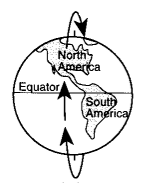
\includegraphics[keepaspectratio,scale=0.75]{June1997-Q56-A}}
      \correctchoice{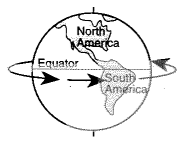
\includegraphics[keepaspectratio,scale=0.75]{June1997-Q56-B}}
        \wrongchoice{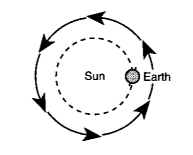
\includegraphics[keepaspectratio,scale=0.75]{June1997-Q56-C}}
        \wrongchoice{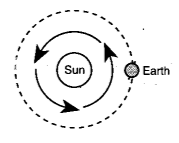
\includegraphics[keepaspectratio,scale=0.75]{June1997-Q56-D}}
    \end{choices}
    \end{multicols}
\end{question}
}

\element{nysed}{
\begin{question}{June1997-Q63}
    The data table below gives the mean radius of orbit ($R$) and the period ($T$) of some planets orbiting the Sun.
    \begin{center}
    \begin{tabu}{X[l]X[c]X[c]}
        %Planet  & Mean Radius of Orbit ($R$) ($\times\SI{e8}{\kilo\meter}$)
        %        & Orbital Period ($T$) (days) \\
        Planet  & $R$ & $T$ \\
        \midrule
        Mercury &  58 &  88 \\
        Venus   & 108 & 225 \\
        Earth   & 150 & 365 \\
        Mars    & 228 & 687 \\
    \end{tabu}
    \end{center}
    Which ratio is constant for these planet?
    \begin{multicols}{4}
    \begin{choices}
        \wrongchoice{$\dfrac{R}{T}$}
        \wrongchoice{$\dfrac{R^2}{T}$}
        \wrongchoice{$\dfrac{R^2}{T^2}$}
      \correctchoice{$\dfrac{R^3}{T^2}$}
    \end{choices}
    \end{multicols}
\end{question}
}

\element{nysed}{
\begin{question}{June1997-Q65}
    The diagram below represents the path of a planet in an elliptical orbit around the Sun.
    \begin{center}
    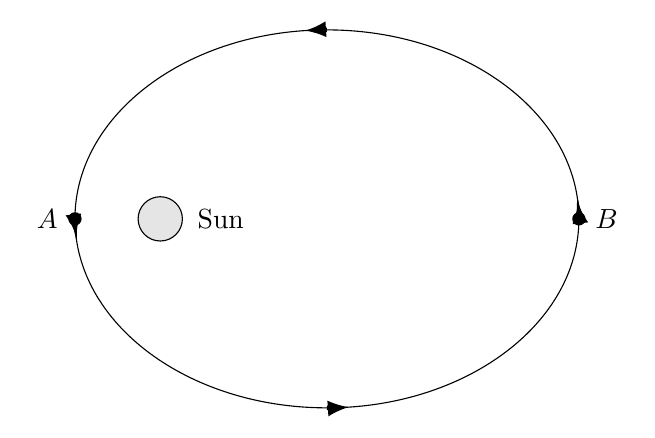
\begin{tikzpicture}[scale=0.8]
        \def\a{4}
        \def\b{3}
        %% orbit
        \draw (0,0) circle (\a{} and \b);
        \foreach \x in {0,90,180,270}
            \draw[ultra thick,-latex] ({\a*cos(\x)},{\b*sin(\x)}) arc (\x:{\x+5}:\a{} and \b);
        %% Sun
        \draw[fill=white!90!black] ({-sqrt(\a*\a-\b*\b)},0) circle (1em) node[anchor=west,xshift=1em] {Sun};
        %% labels
        \foreach \x/\y in {180/A,0/B}
            \fill ({\a*cos(\x)},{\b*sin(\x)}) circle (3pt) node[anchor=center,shift={(\x:1em)}] {$\y$};
    \end{tikzpicture}
    \end{center}
    As the planet moves from point $A$ to point $B$,
        what changes occur in its speed and kinetic energy?
    \begin{choices}
      \correctchoice{Both speed and kinetic energy decrease.}
        \wrongchoice{Both speed and kinetic energy increase.}
        \wrongchoice{Speed decreases and kinetic energy increases.}
        \wrongchoice{Speed increases and kinetic energy decreases.}
    \end{choices}
\end{question}
}


%% Section June1996
%%--------------------
\element{nysed}{
\begin{question}{June1996-Q14}
    A \SI{3.0}{\kilo\gram} mass weighs \SI{15}{\newton} at a given point in the Earth's gravitational field.
    What is the magnitude of the acceleration due to the gravity at this point?
    \begin{multicols}{2}
    \begin{choices}
        \wrongchoice{\SI{45}{\meter\per\second}}
        \wrongchoice{\SI{9.8}{\meter\per\second}}
      \correctchoice{\SI{5.0}{\meter\per\second}}
        \wrongchoice{\SI{0.20}{\meter\per\second}}
    \end{choices}
    \end{multicols}
\end{question}
}

\element{nysed}{
\begin{question}{June1996-Q63}
    The comet Hyakutake, seen in the Earth's sky this year,
        will take more than \num{10 000} years to complete its orbit.
    Which object is at a focus of the comet's orbit?
    \begin{multicols}{2}
    \begin{choices}
        \wrongchoice{Earth}
      \correctchoice{Sun}
        \wrongchoice{Moon}
        \wrongchoice{Jupiter}
    \end{choices}
    \end{multicols}
\end{question}
}

\element{nysed}{
\begin{question}{June1996-Q64}
    The diagram below represents the path of a planet moving in an elliptical orbit around a star.
    The orbital period is of the planet is \SI{10000}{\day}.
    %% NOTE: TODO: finish this
    \begin{center}
    \begin{tikzpicture}
        %% A, B, C, D
        \def\a{4}
        \def\b{3}
        \draw (0,0) circle (\a{} and \b);
        \foreach \x/\y in {355/A,5/B,155/C,204/D}
            \fill ({\a*cos(\x)},{\b*sin(\x)}) circle (2pt) node[anchor=center,shift={(\x:1em)}] {$\y$};
        %% Planet P
        \foreach \x/\y in {300/P}
            \node[anchor=center,fill=white,draw,circle] at ({\a*cos(\x)},{\b*sin(\x)})  {$\y$};
        %% fill areas
        \draw[pattern=north east lines] ({-sqrt(\a*\a-\b*\b)},0) -- ({\a*cos(155)},{\b*sin(155)}) arc(155:204:\a{} and \b) -- cycle;
        \draw[pattern=north east lines] ({-sqrt(\a*\a-\b*\b)},0) -- ({\a*cos(5)},{\b*sin(5)}) arc(5:-5:\a{} and \b) -- cycle;
        %% Sun
        \node[anchor=center,draw,circle,fill=white] at ({-sqrt(\a*\a-\b*\b)},0) {$S$};
    \end{tikzpicture}
    \end{center}
    According to Kepler's laws, how many days are required for the planet to travel from the starting point to point $X$?
    \begin{multicols}{2}
    \begin{choices}
        \wrongchoice{\num{400}}
        \wrongchoice{\num{350}}
        \wrongchoice{\num{300}}
        \wrongchoice{\num{250}}
    \end{choices}
    \end{multicols}
\end{question}
}


%% Section June1994
%%--------------------
\element{nysed}{
\begin{question}{June1994-Q13}
    The magnitude of the gravitational force between two objects is \SI{20}{\newton}.
    If the mass of each object were doubled,
        the magnitude of the gravitational force between the objects would be:
    \begin{multicols}{2}
    \begin{choices}
        \wrongchoice{\SI{5.0}{\newton}}
        \wrongchoice{\SI{10}{\newton}}
        \wrongchoice{\SI{20}{\newton}}
      \correctchoice{\SI{80}{\newton}}
    \end{choices}
    \end{multicols}
\end{question}
}


%% Section June1995
%%--------------------
\element{nysed}{
\begin{question}{June1995-Q63}
    What would occur as a result of the frictional drag of the atmosphere on an artificial satellite orbiting the Earth?
    \begin{choices}
        \wrongchoice{The satellite would increase in speed and escape the gravitational field of the Earth}
        \wrongchoice{The satellite would increase in speed and spiral toward the Earth}
        \wrongchoice{The satellite would decrease in speed and escape the gravitational field of the Earth}
      \correctchoice{The satellite would decrease in speed and spiral toward the Earth}
    \end{choices}
\end{question}
}

\element{nysed}{
\begin{question}{June1995-Q65}
    Satellites $A$ and $B$ are orbiting the Earth in circular orbits as shown below.
    The mass of satellite $A$ is twice as great as the mass of satellite $B$.
    East has radius $R$.
    \begin{center}
    \begin{tikzpicture}
        %% Earth
        \draw[fill=white!90!black] (0,0) circle (0.75);
        \draw[thick,-latex] (0,0) -- (80:0.75) node[pos=0.5,anchor=east] {$R$};
        \node[anchor=north] at (0,-0.75) {Earth};
        %% 2R orbit
        \draw[dashed] (0,0) circle (1.5);
        \node[anchor=center,circle,draw,fill=white,font=\small] at (45:1.5) {$A$};
        \draw[thick,-latex] (0,0) -- (340:1.5) node[pos=0.85,anchor=north east] {$2R$};
        %% 4R orbit
        \draw[dashed] (0,0) circle (3.0);
        \node[anchor=center,circle,draw,fill=white,font=\small] at (330:3.0) {$B$};
        \draw[thick,-latex] (0,0) -- (180:3.0) node[pos=0.75,anchor=south] {$4R$};
    \end{tikzpicture}
    \end{center}
    Compared to the orbital period of satellite $A$,
        the orbital period of satellite $B$ is:
    \begin{multicols}{3}
    \begin{choices}
        \wrongchoice{shorter}
      \correctchoice{longer}
        \wrongchoice{the same}
    \end{choices}
    \end{multicols}
\end{question}
}




%% Section June1990
%%--------------------
\element{nysed}{
\begin{question}{June1990-Q12}
    Two point masses are located a distance, $D$, apart.
    The gravitational force of attraction between them can be quadrupled by changing the distance to:
    \begin{multicols}{2}
    \begin{choices}
      \correctchoice{$\dfrac{D}{2}$}
        \wrongchoice{$2 D$}
        \wrongchoice{$\dfrac{D}{4}$}
        \wrongchoice{$4 D$}
    \end{choices}
    \end{multicols}
\end{question}
}


%% Section June1989
%%--------------------
\element{nysed}{
\begin{question}{June1989-Q13}
    Which graph best represents the relationship between the mass of an object and its distance from the center of the Earth?
    \begin{multicols}{2}
    \begin{choices}
        \AMCboxDimensions{down=-2.5em}
        \wrongchoice{
            \begin{tikzpicture}
                \begin{axis}[
                    axis y line=left,
                    axis x line=bottom,
                    axis line style={->},
                    xlabel={distance},
                    xtick=\empty,
                    ylabel={mass},
                    ytick=\empty,
                    xmin=0,xmax=11,
                    ymin=0,ymax=11,
                    width=\columnwidth,
                    very thin,
                ]
                \addplot[line width=1pt,domain=0:10] {x};
                \end{axis}
            \end{tikzpicture}
        }
        \wrongchoice{
            \begin{tikzpicture}
                \begin{axis}[
                    axis y line=left,
                    axis x line=bottom,
                    axis line style={->},
                    xlabel={distance},
                    xtick=\empty,
                    ylabel={mass},
                    ytick=\empty,
                    xmin=0,xmax=11,
                    ymin=0,ymax=11,
                    width=\columnwidth,
                    very thin,
                ]
                \addplot[line width=1pt,domain=0:10] {10/x};
                \end{axis}
            \end{tikzpicture}
        }
        \wrongchoice{
            \begin{tikzpicture}
                \begin{axis}[
                    axis y line=left,
                    axis x line=bottom,
                    axis line style={->},
                    xlabel={distance},
                    xtick=\empty,
                    ylabel={mass},
                    ytick=\empty,
                    xmin=0,xmax=11,
                    ymin=0,ymax=11,
                    width=\columnwidth,
                    very thin,
                ]
                \addplot[line width=1pt,domain=0:10] {0.1*x*x};
                \end{axis}
            \end{tikzpicture}
        }
        %% ANS is 4
        \correctchoice{
            \begin{tikzpicture}
                \begin{axis}[
                    axis y line=left,
                    axis x line=bottom,
                    axis line style={->},
                    xlabel={distance},
                    xtick=\empty,
                    ylabel={mass},
                    ytick=\empty,
                    xmin=0,xmax=11,
                    ymin=0,ymax=11,
                    width=\columnwidth,
                    very thin,
                ]
                \addplot[line width=1pt,domain=0:10] {6};
                \end{axis}
            \end{tikzpicture}
        }
    \end{choices}
    \end{multicols}
\end{question}
}

\element{nysed}{
\begin{question}{June1989-Q14}
    Gravitational force of attraction $F$ exists between two point masses $A$ and $B$ when they are separated by a fixed distance.
    After mass $A$ is tripled and mass $B$ is halved,
        the gravitational attraction between the two masses is:
    \begin{multicols}{2}
    \begin{choices}
        \wrongchoice{$\dfrac{F}{6}$}
        \wrongchoice{$\dfrac{3F}{2}$}
      \correctchoice{$\dfrac{2F}{3}$}
        \wrongchoice{$6F$}
    \end{choices}
    \end{multicols}
\end{question}
}


\element{nysed}{
\begin{question}{June1989-Q64}
    The path of a satellite orbiting the Earth is best described as:
    \begin{multicols}{2}
    \begin{choices}
        \wrongchoice{linear}
        \wrongchoice{hyperbolic}
        \wrongchoice{parabolic}
      \correctchoice{elliptical}
    \end{choices}
    \end{multicols}
\end{question}
}

\element{nysed}{
\begin{question}{June1989-Q66}
    Four planets orbiting the Sun,
        the ratio of the mean radius of the orbit cubed to the orbital period of motion squared is:
    \begin{choices}
        \wrongchoice{greatest for the most massive planet}
        \wrongchoice{greatest for the least massive planet}
        \wrongchoice{constantly changing as a planet rotates}
      \correctchoice{the same for all planets}
    \end{choices}
\end{question}
}

\element{nysed}{
\begin{question}{June1989-Q67}
    A satellite orbits the Earth in a circular orbit.
    Which statement best explains why the satellite does not move closer to the center of the Earth?
    \begin{choices}
        \wrongchoice{The gravitational field of the Earth does not reach the satellite's orbit}
        \wrongchoice{The Earth's gravity keeps the satellite moving with constant velocity}
      \correctchoice{The satellite is always moving perpendicularly to the force due to gravity}
        \wrongchoice{The satellite does not have any weight}
    \end{choices}
\end{question}
}

\element{nysed}{
\begin{question}{June1989-Q68}
    Which condition is required for a satellite to be in a geosynchronous orbit about the Earth?
    \begin{choices}
      \correctchoice{The period of revolution of the satellite must be the same as the rotational period of the Earth.}
        \wrongchoice{The altitude of the satellite must be equal to the radius of the Earth.}
        \wrongchoice{The orbital speed of the satellite around the Earth must be the same as the orbital speed of the Earth around the Sun.}
        \wrongchoice{The daily distance traveled by the satellite must be equal to the circumference of the Earth.}
    \end{choices}
\end{question}
}

\element{nysed}{
\begin{question}{June1989-Q70}
    The diagram below shows the movement of a planet around the Sun.
    Area 1 equals area 2.
    \begin{center}
    \begin{tikzpicture}
        \def\a{3}\def\b{2.5}
        \def\f{{sqrt((\a*\a)-(\b*\b))}}
        %% orbit
        \draw (0,0) circle (\a{} and \b);
        \draw[thick,-latex] (\a,0) arc(0:120:\a{} and \b);
        \draw[thick,-latex] (-\a,0) arc(180:300:\a{} and \b);
        %% A, B, C, D
        \foreach \x/\y in {355/A,5/B,163/C,197/D}
            \fill ({\a*cos(\x)},{\b*sin(\x)}) circle (2pt) node[anchor=center,shift={(\x:1em)}] {$\y$};
        %% Region 1 and 2
        \draw[pattern=north east lines] ({\a*cos(5)},{\b*sin(5)}) arc(5:-5:\a{} and \b) to (-\f,0) -- cycle;
        \path (-\f,0) -- ++(5:\a) node[anchor=south] {2};
        \draw[pattern=north east lines] ({\a*cos(163)},{\b*sin(163)}) arc(163:197:\a{} and \b) to (-\f,0) -- cycle;
        \node[anchor=center] at (-\b,0) {1};
        %% sun
        \draw[fill=white] (-\f,0) circle (1ex);
        \node[pin={300:Sun}] at (-\f,0) {};
        %% planet
        \fill (0,2.5) circle (1ex);
        \node[pin={30:planet}] at (0,2.5) {};
    \end{tikzpicture}
    \end{center}
    Compared to the time the planet takes to move from $C$ to $D$,
        the time it takes to move from $A$ to $B$ is:
    \begin{multicols}{3}
    \begin{choices}
        \wrongchoice{less}
        \wrongchoice{greater}
      \correctchoice{the same}
    \end{choices}
    \end{multicols}
\end{question}
}


%% Section June1986
%%--------------------
\element{nysed}{
\begin{question}{June1986-Q09}
    Which graph best represents the gravitational force between two point masses as a function of the distance between the masses?
    \begin{multicols}{2}
    \begin{choices}
        \AMCboxDimensions{down=-2.5em}
        \wrongchoice{
            \begin{tikzpicture}
                \begin{axis}[
                    axis y line=left,
                    axis x line=bottom,
                    axis line style={->},
                    xlabel={distance},
                    xtick=\empty,
                    ylabel={force},
                    ytick=\empty,
                    xmin=0,xmax=11,
                    ymin=0,ymax=11,
                    width=\columnwidth,
                    very thin,
                ]
                \addplot[line width=1pt,domain=0:10]{x};
                \end{axis}
            \end{tikzpicture}
        }
        \wrongchoice{
            \begin{tikzpicture}
                \begin{axis}[
                    axis y line=left,
                    axis x line=bottom,
                    axis line style={->},
                    xlabel={distance},
                    xtick=\empty,
                    ylabel={force},
                    ytick=\empty,
                    xmin=0,xmax=11,
                    ymin=0,ymax=11,
                    width=\columnwidth,
                    very thin,
                ]
                \addplot[line width=1pt,domain=0:10]{0.1*x*x};
                \end{axis}
            \end{tikzpicture}
        }
        %% ANS is 3
        \correctchoice{
            \begin{tikzpicture}
                \begin{axis}[
                    axis y line=left,
                    axis x line=bottom,
                    axis line style={->},
                    xlabel={distance},
                    xtick=\empty,
                    ylabel={force},
                    ytick=\empty,
                    xmin=0,xmax=11,
                    ymin=0,ymax=11,
                    width=\columnwidth,
                    very thin,
                ]
                \addplot[line width=1pt,domain=0:10]{10/x};
                \end{axis}
            \end{tikzpicture}
        }
        \wrongchoice{
            \begin{tikzpicture}
                \begin{axis}[
                    axis y line=left,
                    axis x line=bottom,
                    axis line style={->},
                    xlabel={distance},
                    xtick=\empty,
                    ylabel={force},
                    ytick=\empty,
                    xmin=0,xmax=11,
                    ymin=0,ymax=11,
                    width=\columnwidth,
                    very thin,
                ]
                \addplot[line width=1pt,domain=0:10]{sqrt(10)*sqrt(x)};
                \end{axis}
            \end{tikzpicture}
        }
    \end{choices}
    \end{multicols}
\end{question}
}


%% Section June1985
%%--------------------
\element{nysed}{
\begin{question}{June1985-Q08}
    Two objects of fixed mass are moved apart so that they are separated by three times their original distance.
    Compared to the original gravitational force between then,
        the new gravitational force is:
    \begin{multicols}{2}
    \begin{choices}
        \wrongchoice{one-third as great}
      \correctchoice{one-ninth as great}
        \wrongchoice{three times as great}
        \wrongchoice{nine times as great}
    \end{choices}
    \end{multicols}
\end{question}
}



\endinput


